% tex file for regression results
\par To develop linear models, we looked at the HR from the neural response 
as a single feature. Originally we used multiple regression to take into 
account the 3 different types of stimulus (pump, explode, cash-out) to see if 
the separation of these stimuli can better describe the response, but it wasn't 
that good. In figure \ref{fig:all_cond_time}, we can see the different 
conditions broken up. Using smoothed data, fourier and drift features in linear 
regression we obtained fitted values for fMRI BOLD contrast of a random 
voxel and also calculated the residuals for a random voxel for subject 001, 
voxel $(30,40,15)$ [Figure \ref{fig:fit_vs_act}, \ref{fig:fit_vs_res}].

  
\begin{figure}[ht]
\centering
\begin{minipage}[b]{0.45\linewidth}
	\centering
	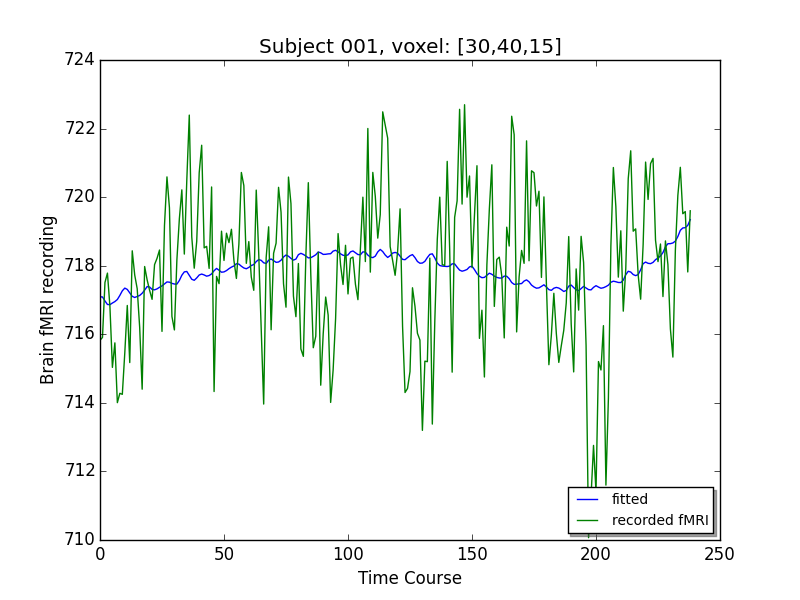
\includegraphics[width=.8\linewidth]{../images/Fitted_v_Actual.png} 
	\caption{Fitted/Predicted vs Actual fMRI BOLD contrast}
	\label{fig:fit_vs_act}
\end{minipage}	
\quad
\begin{minipage}[b]{0.45\linewidth}
	\centering
		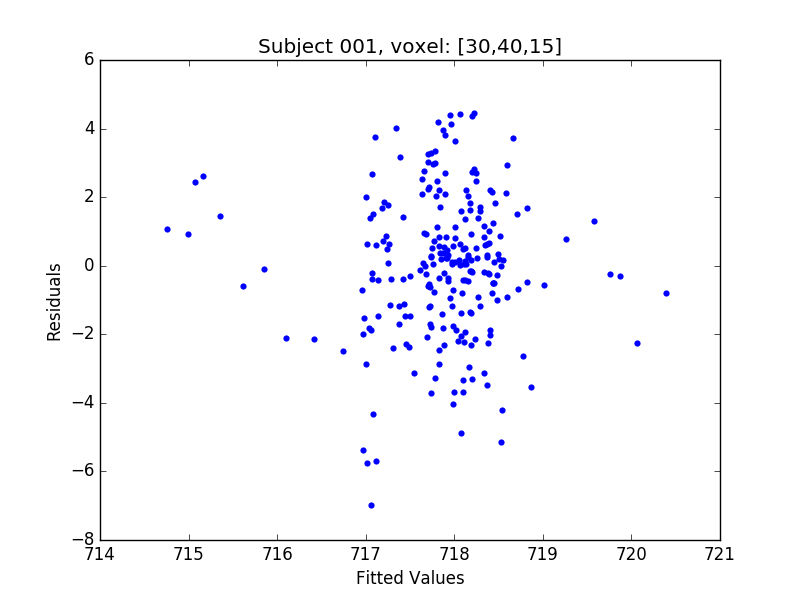
\includegraphics[width=.8\linewidth]{../images/Fitted_v_Residuals.png} 
	\caption{Fitted fMRI BOLD contrast vs Residual from Linear Regression}
	\label{fig:fit_vs_res}
\end{minipage}
\end{figure}




%\begin{figure}[ht]
%\centering
%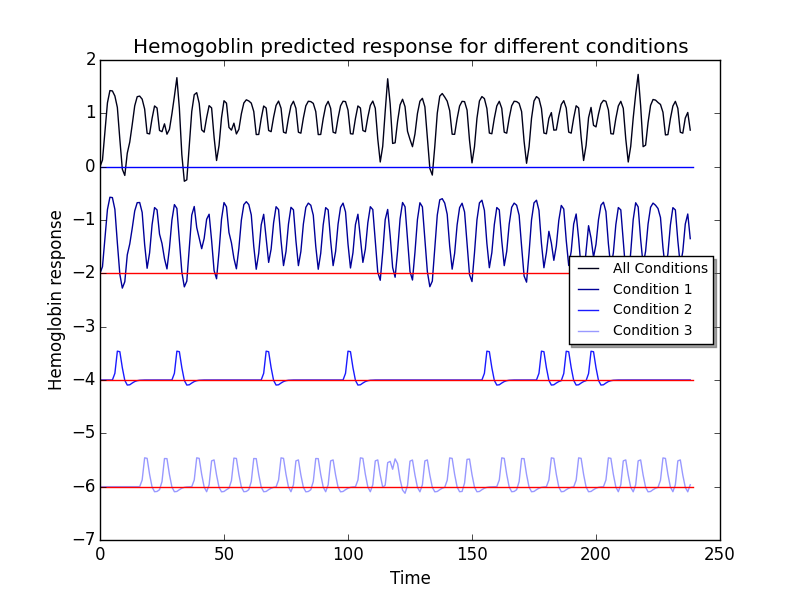
\includegraphics[scale=.5]{../images/all_cond_time}  
%\caption{Plotting all predicted HR for conditions.}
%\label{fig:all_cond_time}
%\end{figure}

*****As we also obtained $\hat{\beta}$ values (coefficients) from the linear 
regression models, we looked at the 3-dimensional reports of the 
$\hat{\beta}$ values, a less rigorous analysis than hypothesis testing with 
t-statistics [Figure reference]. $\sim$Remove or update****



The numerous other multiple regression models discussed in 
\textit{Linear Regression} should be analyzed similarly in the future. 
